\documentclass[11pt,a4paper]{article}
\usepackage[margin=1in]{geometry}
\usepackage{booktabs}
\usepackage{array}
\usepackage{longtable}
\usepackage{enumitem}
\usepackage{xcolor}
\usepackage{listings}
\usepackage{tikz}
\usetikzlibrary{arrows.meta,positioning,shapes.geometric,fit,calc}
\usepackage{amsmath}
\usepackage{amssymb}
\usepackage{hyperref}
\hypersetup{colorlinks=true, linkcolor=blue!60!black, urlcolor=blue!60!black}

\definecolor{codebg}{gray}{0.95}
\lstset{
  basicstyle=\ttfamily\small,
  backgroundcolor=\color{codebg},
  frame=single,
  framerule=0pt,
  breaklines=true,
}

\newcommand{\code}[1]{\texttt{#1}}
\newcolumntype{L}[1]{>{\raggedright\arraybackslash}p{#1}}

\title{Mesh Agent Architecture:\\Backends, Routing, Tools, and Memory}
\author{Reference Document --- \code{hello-world} Mesh System}
\date{May 2026}

\begin{document}
\maketitle

\begin{abstract}
This document describes the architecture of the \code{hello-world} mesh
agent system, covering five layers: LLM backend dispatch, tool routing
through \code{complete\_with\_tools}, the harness tool surface used by
the plan-and-execute controller, security hardening of subprocess and
credential handling, and the episodic memory system (formation,
curation, and retrieval). Configuration lives in \code{mesh.yaml};
runtime dispatch lives in \code{mesh/llm.py}; memory state lives in
\code{\textasciitilde/.mesh/memory/}.
\end{abstract}

\tableofcontents
\newpage

%----------------------------------------------------------------------
\section{System Overview}
%----------------------------------------------------------------------

The mesh is a multi-agent system where a central \textbf{router}
classifies user messages and either responds directly or dispatches work
to agent nodes.  The router has its own LLM backend
(\code{router\_v2\_llm\_backend}) and runs a state machine
(IDLE\,/\,BUSY) that is distinct from any worker LLM.

Each agent node has:
\begin{itemize}[nosep]
  \item An \textbf{LLM backend} (how it calls language models),
  \item A \textbf{tool surface} (what tools are available),
  \item An optional \textbf{harness layer} (plan-and-execute controller).
\end{itemize}

\begin{figure}[h]
\centering
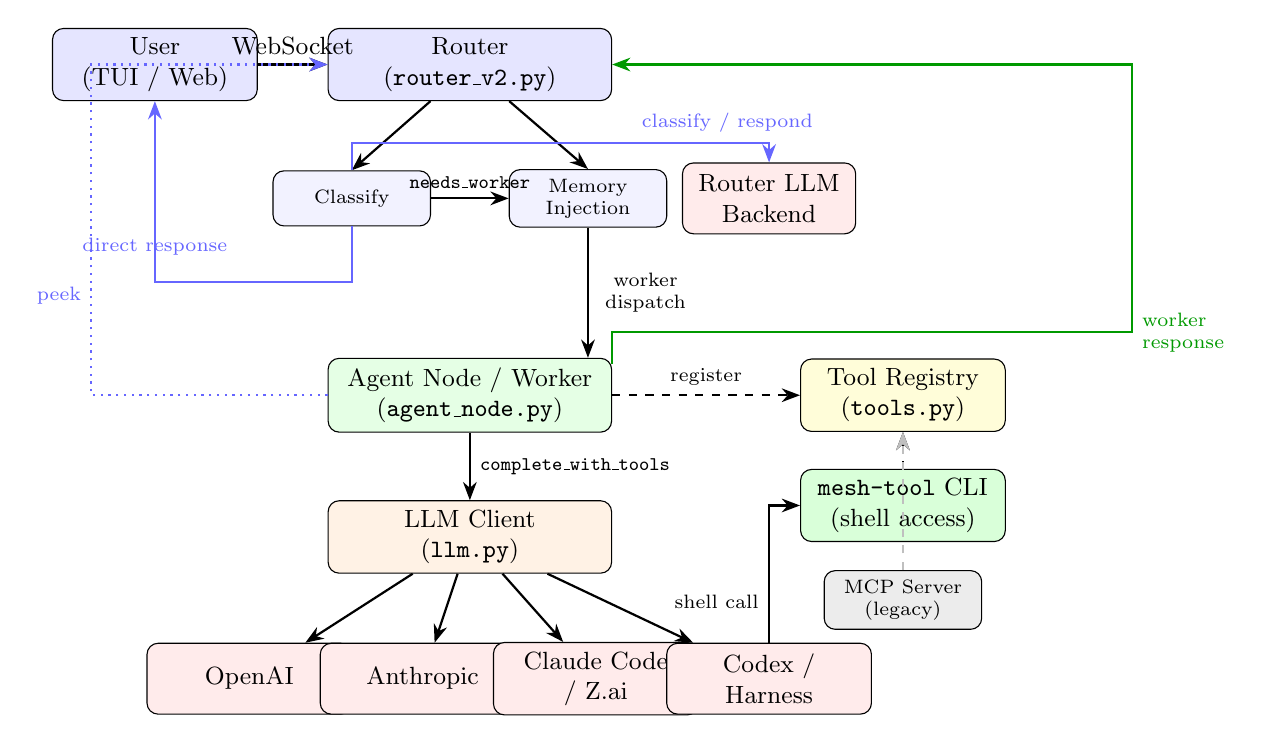
\begin{tikzpicture}[
    >=Stealth,
    box/.style={draw, rounded corners, minimum height=0.9cm,
                minimum width=2.6cm, align=center, font=\small},
    wide/.style={box, minimum width=3.6cm},
    smallbox/.style={draw, rounded corners, minimum height=0.7cm,
                     minimum width=2cm, align=center,
                     font=\scriptsize},
    arrow/.style={->, thick},
    dasharrow/.style={->, thick, dashed},
    every node/.style={font=\small},
  ]

  % ══════════════════════════════════════════════
  % Layout — five columns, five rows
  %
  %   x=0    : User (row 0), peek path (rows 1-2)
  %   x=4    : Router (row 0), Classify (row 1)
  %   x=6.8  : MemInj (row 1), Router LLM Backend (row 1, far right)
  %   x=4.5  : Agent (row 2), LLM Client (row 3), Backends (row 4)
  %   x=10   : Tools column (rows 2-4)
  % ══════════════════════════════════════════════

  % ── Row 0: User + Router ──
  \node[box, fill=blue!10] at (0, 0) (user) {User\\(TUI / Web)};
  \node[wide, fill=blue!10] at (4, 0) (router)
    {Router\\(\code{router\_v2.py})};

  % ── Row 1: Router internals + Router's own LLM backend ──
  \node[smallbox, fill=blue!5] at (2.5, -1.7) (classify)
    {Classify};
  \node[smallbox, fill=blue!5] at (5.5, -1.7) (meminj)
    {Memory\\Injection};
  \node[box, fill=red!8, minimum width=2.2cm] at (7.8, -1.7)
    (routerllm) {Router LLM\\Backend};

  % ── Row 2: Agent Node ──
  \node[wide, fill=green!10] at (4, -4.2) (agent)
    {Agent Node / Worker\\(\code{agent\_node.py})};

  % ── Row 3: Worker LLM Client ──
  \node[wide, fill=orange!10] at (4, -6) (llm)
    {LLM Client\\(\code{llm.py})};

  % ── Row 4: Backends ──
  \node[box, fill=red!8] at (1.2, -7.8) (openai) {OpenAI};
  \node[box, fill=red!8] at (3.4, -7.8) (anthropic) {Anthropic};
  \node[box, fill=red!8] at (5.6, -7.8) (cc) {Claude Code\\/ Z.ai};
  \node[box, fill=red!8] at (7.8, -7.8) (other) {Codex /\\Harness};

  % ── Tools column (right side, rows 2-4) ──
  \node[box, fill=yellow!15] at (9.5, -4.2) (tools)
    {Tool Registry\\(\code{tools.py})};
  \node[box, fill=green!15] at (9.5, -5.6) (meshtool)
    {\code{mesh-tool} CLI\\(shell access)};
  \node[smallbox, fill=gray!15] at (9.5, -6.8) (mcp)
    {MCP Server\\(legacy)};

  % ══════════════════════════════════════════════
  % Arrows — routed to avoid crossing any nodes
  % ══════════════════════════════════════════════

  % ── User ↔ Router (clean horizontal, top row) ──
  \draw[arrow] (user) -- node[above] {WebSocket} (router);

  % ── Router → internals (short drops from router bottom) ──
  \draw[arrow] ([xshift=-5mm]router.south) -- (classify.north);
  \draw[arrow] ([xshift=5mm]router.south) -- (meminj.north);

  % ── Classify → needs_worker → Memory Injection (horizontal) ──
  \draw[arrow] (classify) -- node[above, font=\scriptsize]
    {\code{needs\_worker}} (meminj);

  % ── Classify → Router LLM Backend ──
  % Route above the row-1 boxes via an L-shape
  \draw[arrow, blue!60]
    (classify.north) -- ++(0, 0.35)
    -| node[pos=0.45, above, font=\scriptsize]
    {classify / respond} (routerllm.north);

  % ── Direct response: classify → user ──
  % Drop below row 1, go left to x=0, up into user.south.
  % Stays between rows 1 and 2 — clear of agent node.
  \draw[arrow, blue!60]
    (classify.south) -- ++(0, -0.7)
    -| node[pos=0.65, below, font=\scriptsize]
    {direct response} (user.south);

  % ── BUSY-state peek: agent → router ──
  % Far-left margin (x ≈ −1), clear of direct-response path at x=0
  \draw[arrow, blue!60, dotted]
    (agent.west) -- ++(-3, 0)
    |- node[pos=0.15, left, font=\scriptsize] {peek}
    (router.west);

  % ── Memory Injection → Agent Node (straight down) ──
  \draw[arrow] (meminj.south) --
    node[right, font=\scriptsize, text width=1.2cm, align=center]
    {worker\\dispatch}
    (agent.north -| meminj);

  % ── Agent → Worker LLM Client (straight down) ──
  \draw[arrow] (agent) -- node[right, font=\scriptsize]
    {\code{complete\_with\_tools}} (llm);

  % ── Worker LLM → Backends (fan out) ──
  \draw[arrow] (llm) -- (openai);
  \draw[arrow] (llm) -- (anthropic);
  \draw[arrow] (llm) -- (cc);
  \draw[arrow] (llm) -- (other);

  % ── Agent → Tool Registry (horizontal right) ──
  \draw[dasharrow] (agent) -- node[above, font=\scriptsize]
    {register} (tools);

  % ── Codex/Harness → mesh-tool (up from other, right to meshtool) ──
  % Routes LEFT of the tools column — avoids crossing MCP box
  \draw[arrow] (other.north) |- node[pos=0.15, left,
    font=\scriptsize] {shell call} (meshtool.west);

  % ── mesh-tool → Tool Registry ──
  \draw[dasharrow] (meshtool) -- (tools);

  % ── Legacy MCP → Tool Registry (faded) ──
  \draw[dasharrow, gray!50] (mcp) -- (tools);

  % ── Worker completion response: Agent → Router → User ──
  % Route above Tool Registry (y ≈ -3.4) to the right margin (x ≈ 12),
  % then up to router level.  Avoids crossing Tool Registry at y=-4.2.
  \draw[arrow, green!60!black]
    ([yshift=4mm]agent.east) -- ++(0, 0.4)
    -- ++(6.6, 0)
    node[right, font=\scriptsize, text width=1.3cm, align=left]
      {worker\\response}
    |- (router.east);

\end{tikzpicture}
\caption{Message flow through the mesh.  The router has its own LLM
backend (\code{router\_v2\_llm\_backend}, separate from the worker's)
used for classification and direct response generation (blue arrows).
On \code{needs\_worker}, the router injects relevant memories and
dispatches to the agent node, which calls its own LLM backend via
\code{complete\_with\_tools}.  While a worker is running (BUSY), the
router generates interim responses via worker peek (dotted blue line).
When the worker completes, the agent node sends the response back
through the router to the user (green arrow, right side).
Codex\,/\,Harness subprocesses access mesh tools via the
\code{mesh-tool} CLI.  Dashed lines indicate tool discovery; gray
indicates legacy paths.}
\label{fig:overview}
\end{figure}

\paragraph{Router states.}
RouterV2 operates a two-state machine:
\begin{description}[nosep, leftmargin=1.5em, labelwidth=1.2em]
  \item[IDLE] Incoming message $\to$ LLM classification call $\to$
    \code{\{needs\_response, needs\_worker\}}.  If
    \code{needs\_worker} is false, the router generates a direct
    response and stays IDLE.  If true, the router sends an immediate
    acknowledgment, injects relevant memories
    (\S\ref{sec:harness-toolset}), and spawns a worker.
  \item[BUSY] Worker is running.  New messages are handled by the
    router's own LLM, which peeks at the worker's in-progress
    context to generate contextual interim responses.
\end{description}

\noindent RouterV3 extends this with a planning pipeline---an
additional router-level LLM loop that generates and validates a plan
before worker dispatch.

%----------------------------------------------------------------------
\section{LLM Backends}
\label{sec:backends}
%----------------------------------------------------------------------

Backends are configured in \code{mesh.yaml} under \code{llm\_backends:}
and assigned to agents via the \code{llm\_backend} field on each node.
The \code{LLMClient} class in \code{mesh/llm.py} dispatches to a
backend-specific completion method based on \code{LLMConfig.backend}.

\subsection{Backend Types}

\begin{table}[h]
\centering
\small
\begin{tabular}{@{}llL{6.5cm}@{}}
\toprule
\textbf{Type} & \textbf{Method} & \textbf{Notes} \\
\midrule
\code{openai}
  & \code{\_complete\_openai} /
    \code{\_complete\_openai\_responses}
  & Two paths: Chat Completions API for standard models;
    Responses API for reasoning models (detected via
    \code{should\_use\_responses\_api}). Supports native
    function calling. \\
\addlinespace
\code{anthropic}
  & \code{\_complete\_anthropic}
  & Claude API with native \code{tool\_use} blocks. Supports
    vision (image extraction from history). \\
\addlinespace
\code{claude-code}
  & \code{\_complete\_claude\_code}
  & Claude Code CLI subprocess. Supports MCP sidecar for
    mesh tools. Multi-account fallback via
    \code{cc\_fallback\_homes}. \\
\addlinespace
\code{zai}
  & \code{\_complete\_zai}
  & Z.ai proxy. Same interface as \code{claude-code}
    (MCP sidecar, CC CLI subprocess). \\
\addlinespace
\code{codex}
  & \code{\_complete\_codex}
  & Codex CLI subprocess with its own built-in tool loop
    (\code{codex:shell}, \code{codex:patch}, etc.).
    Mesh tools available via \code{mesh-tool} CLI on
    \code{PATH} (repo root prepended to subprocess env). \\
\addlinespace
\code{mesh-harness}
  & \code{\_complete\_mesh\_harness}
  & Standalone TAOR (think-act-observe-reflect) loop
    as a subprocess. Usable as any agent backend, not
    only for plan-and-execute. Tool set is configurable
    via \code{harness\_toolset} (see
    \S\ref{sec:harness-toolset}). \\
\bottomrule
\end{tabular}
\caption{LLM backend types and their dispatch methods.}
\label{tab:backends}
\end{table}

\subsection{Live Backend Examples}

The production \code{mesh.yaml} defines $\sim$40 backend configurations.
Representative examples:

\begin{table}[h]
\centering
\small
\begin{tabular}{@{}llll@{}}
\toprule
\textbf{Name} & \textbf{Type} & \textbf{Model} & \textbf{Use Case} \\
\midrule
\code{default}              & openai     & gpt-5.1              & General agents \\
\code{openai-reasoning-*}   & openai     & o4-mini / o3         & Reasoning tasks \\
\code{claude-code-opus}     & claude-code & opus                & Most agents \\
\code{deepseek-direct}      & openai     & deepseek-v4-flash    & Memory formation \\
\code{codex-5.5}            & codex      & gpt-5.5              & Codex agents \\
\code{mesh-harness-glm51-pe}& mesh-harness & GLM-5.1 + DS-pro  & Plan-and-execute \\
\bottomrule
\end{tabular}
\caption{Selected backend configurations from production \code{mesh.yaml}.}
\end{table}

%----------------------------------------------------------------------
\section{Tool Routing: \code{complete\_with\_tools}}
\label{sec:tool-routing}
%----------------------------------------------------------------------

The central dispatch method is \code{LLMClient.complete\_with\_tools()}
in \code{mesh/llm.py}. It accepts a \code{ToolRegistry}, a list of
enabled tool names, and optional MCP configuration, then routes based on
backend type.

\subsection{Dispatch Paths}

\begin{figure}[h]
\centering
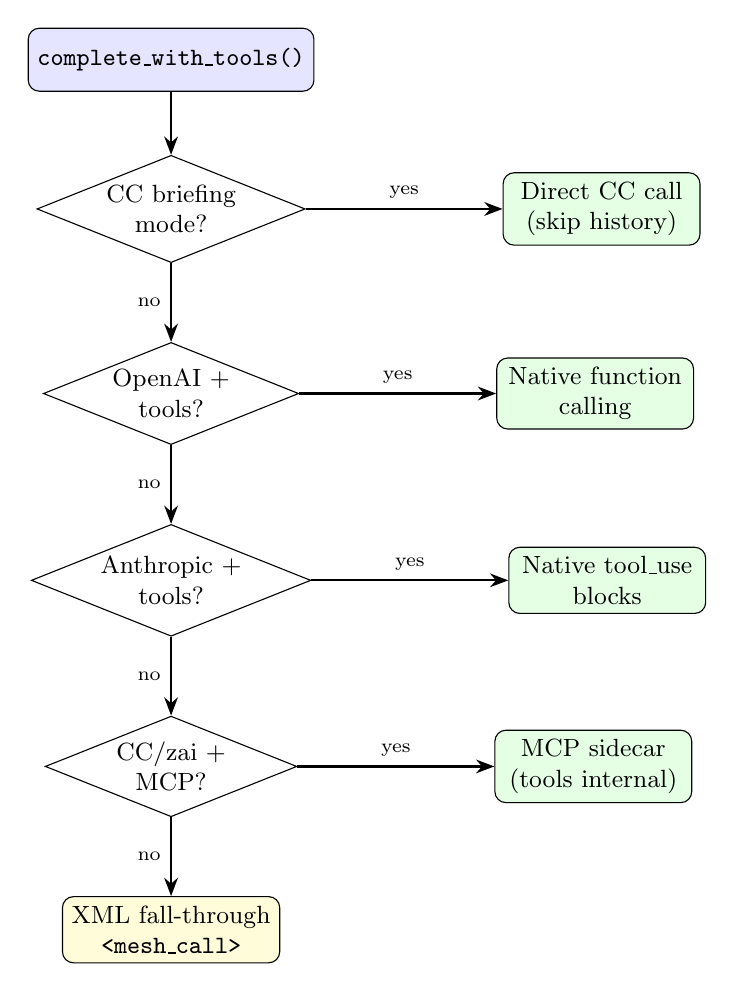
\begin{tikzpicture}[
    >=Stealth,
    decision/.style={diamond, draw, aspect=2.5, inner sep=1pt,
                     font=\small, align=center},
    block/.style={draw, rounded corners, minimum height=0.8cm,
                  minimum width=2.5cm, font=\small, align=center},
    arrow/.style={->, thick},
  ]

  \node[block, fill=blue!10] (entry) {\code{complete\_with\_tools()}};

  \node[decision, below=0.8cm of entry] (d1)
    {CC briefing\\mode?};

  \node[block, fill=green!10, right=2.5cm of d1] (brief)
    {Direct CC call\\(skip history)};

  \node[decision, below=1cm of d1] (d2)
    {OpenAI +\\tools?};

  \node[block, fill=green!10, right=2.5cm of d2] (oai)
    {Native function\\calling};

  \node[decision, below=1cm of d2] (d3)
    {Anthropic +\\tools?};

  \node[block, fill=green!10, right=2.5cm of d3] (ant)
    {Native tool\_use\\blocks};

  \node[decision, below=1cm of d3] (d4)
    {CC/zai +\\MCP?};

  \node[block, fill=green!10, right=2.5cm of d4] (mcp)
    {MCP sidecar\\(tools internal)};

  \node[block, fill=yellow!15, below=1cm of d4] (xml)
    {XML fall-through\\\code{<mesh\_call>}};

  \draw[arrow] (entry) -- (d1);
  \draw[arrow] (d1) -- node[above, font=\scriptsize] {yes} (brief);
  \draw[arrow] (d1) -- node[left, font=\scriptsize] {no} (d2);
  \draw[arrow] (d2) -- node[above, font=\scriptsize] {yes} (oai);
  \draw[arrow] (d2) -- node[left, font=\scriptsize] {no} (d3);
  \draw[arrow] (d3) -- node[above, font=\scriptsize] {yes} (ant);
  \draw[arrow] (d3) -- node[left, font=\scriptsize] {no} (d4);
  \draw[arrow] (d4) -- node[above, font=\scriptsize] {yes} (mcp);
  \draw[arrow] (d4) -- node[left, font=\scriptsize] {no} (xml);

\end{tikzpicture}
\caption{Decision tree in \code{complete\_with\_tools}. The first
matching branch is taken; unmatched backends fall through to XML.}
\label{fig:dispatch}
\end{figure}

\begin{table}[h]
\centering
\small
\begin{tabular}{@{}lL{3cm}L{3.5cm}L{3.5cm}@{}}
\toprule
\textbf{Path} & \textbf{Condition} & \textbf{Tool Format} & \textbf{Response Parsing} \\
\midrule
CC briefing
  & \code{cc\_system\_prompt} \& \code{cc\_user\_prompt} set,
    backend $\in$ \{cc, zai\}
  & None (worker dispatch)
  & Plain text, no tool calls \\
\addlinespace
OpenAI native
  & \code{backend == "openai"} \& tools
  & \code{get\_openai\_tools()} or \code{get\_openai\_responses\_tools()}
  & \code{\_convert\_openai\_tool\_calls()} \\
\addlinespace
Anthropic native
  & \code{backend == "anthropic"} \& tools
  & \code{get\_anthropic\_tools()}
  & \code{\_convert\_openai\_tool\_calls()} \\
\addlinespace
CC/zai + MCP
  & backend $\in$ \{cc, zai\} \& \code{mcp\_config}
    \textbf{[Legacy]}
  & MCP sidecar (tools internal to CC)
  & Plain text; CC executes tools internally.
    Being replaced by \code{mesh-tool} CLI. \\
\addlinespace
XML fall-through
  & Codex, harness, CC/zai without MCP
    \textbf{[Legacy]}
  & \code{format\_tools\_prompt()} $\to$ XML \code{<mesh\_call>} in prompt
  & \code{parse\_tool\_calls()} regex on response.
    Emits \code{DeprecationWarning}. \\
\bottomrule
\end{tabular}
\caption{Tool routing paths in \code{complete\_with\_tools}.}
\label{tab:dispatch}
\end{table}

\subsection{Tool Format Conversion}

The \code{ToolRegistry} (in \code{mesh/tools.py}) provides format
converters for each backend:

\begin{itemize}[nosep]
  \item \code{get\_openai\_tools()} --- OpenAI Chat Completions
        function calling format.
  \item \code{get\_openai\_responses\_tools()} --- OpenAI Responses API
        flattened tool format.
  \item \code{get\_anthropic\_tools()} --- Anthropic \code{tool\_use}
        format.
  \item \code{format\_tools\_prompt()} --- XML
        \code{<mesh\_call>} prompt block for completion-only backends.
\end{itemize}

\subsection{\code{mesh-tool} CLI (Primary Path)}
\label{sec:mesh-tool}

The \code{mesh-tool} CLI provides shell-based access to mesh tools,
replacing the MCP sidecar for all backends with shell access. Any agent
that can execute shell commands can call mesh tools directly---no schema
injection, XML parsing, or MCP plumbing required.

\paragraph{Architecture.}
\code{mesh-tool} is a bash wrapper at the repository root that activates
the virtualenv and runs \code{python -m mesh.cli.mesh\_tool}. It imports
the same \code{tool\_implementations.py} functions used by the
\code{ToolRegistry}---no reimplementation.

\begin{lstlisting}
mesh-tool (bash wrapper, repo root)
  -> python -m mesh.cli.mesh_tool
     -> imports mesh.tool_implementations
     -> looks up tool in ToolRegistry
     -> parses --key value args (type coercion)
     -> executes handler (async-aware)
     -> JSON to stdout, errors to stderr
\end{lstlisting}

\paragraph{Invocation contract.}
\begin{itemize}[nosep]
  \item \code{mesh-tool} (no args) --- lists all available tools grouped
        by category.
  \item \code{mesh-tool <name>} (no required args provided) --- prints
        usage with required/optional parameters.
  \item \code{mesh-tool <name> -{}-help} --- same as above.
  \item \code{mesh-tool <name> -{}-arg value ...} --- executes the tool.
  \item Wrong/missing arguments --- prints error to stderr with
        ``Did you mean?'' suggestions, usage to stdout, exit~1.
\end{itemize}

\paragraph{Output contract.}
\begin{itemize}[nosep]
  \item \textbf{Success}: JSON to stdout, exit~0.
  \item \textbf{Error}: human-readable message to stderr, usage to
        stdout, exit~1.
  \item \textbf{Help}: usage text to stdout, exit~0.
\end{itemize}

\paragraph{Identity.}
The environment variable \code{MESH\_NODE\_ID} identifies the calling
agent (e.g., \code{agent:sysadmin:bob}). It is propagated through two
layers: (1)~\code{os.environ} is set at agent construction for tool
subprocess inheritance (\code{bash\_exec}, etc.); (2)~\code{LLMConfig.node\_id}
is threaded explicitly into each LLM subprocess environment
(\code{\_run\_cc\_subprocess}, \code{\_complete\_codex},
\code{\_complete\_mesh\_harness}). The explicit path ensures correctness
if multiple agents share a process.

\paragraph{PATH wiring.}
The agent runtime prepends the repository root to \code{PATH} in both
\code{\_run\_cc\_subprocess()} and \code{\_complete\_codex()}, making
\code{mesh-tool} discoverable by any subprocess spawned by these
backends.

\paragraph{Prompt injection.}
All agent prompts auto-include \code{mesh/prompts/mesh\_tools.md} via
the \code{load\_prompt\_file()} auto-include mechanism (same pattern as
\code{channel\_policy.md} and \code{memory.md}). This gives agents
concise instructions on discovering and calling mesh-tool from the shell.

\paragraph{Tool surface.}
37~read-only tools across Gmail, web search, notes, literature,
calendar, memory, maps, mesh info, finance, and utility categories.
Plus \code{send\_message} for agent communication.

\paragraph{Agent-routed tools.}
Tools requiring agent-local state (\code{send\_message},
\code{channel\_list}, \code{mesh\_status}, \code{agent\_status},
\code{schedule\_wake}, etc.) are dispatched via the agent's Unix socket
at \code{\textasciitilde/.mesh/sockets/\{sanitized\_id\}.sock}
(directory mode~0700, owner-only access). The CLI falls back to the
legacy \code{/tmp/mesh\_agent\_*} path for agents started before the
hardening change. Memory tools also prefer the socket path when
available.

\paragraph{Confirmation-gated tools.}
Write operations (\code{gmail\_send\_message},
\code{calendar\_create\_event}, \code{gmail\_reply\_to},
\code{calendar\_delete\_event}) are currently excluded from the
\code{mesh-tool} surface. They will be added with a dedicated
confirmation mechanism in a future iteration.

\subsection{MCP Bridge (Legacy)}
\label{sec:mcp}

\textbf{Status: Being replaced by \code{mesh-tool} CLI
(\S\ref{sec:mesh-tool}).} The MCP sidecar is still functional but is no
longer the recommended path. New agents should use \code{mesh-tool} via
shell instead.

For \code{claude-code} and \code{zai} backends, mesh tools were
historically exposed via an MCP (Model Context Protocol) server sidecar
defined in \code{mesh/mcp\_server.py}. The CC subprocess is started with
\code{-{}-mcp-config} pointing to a temporary JSON file that configures
the MCP server.

\paragraph{Agent-local tools.}
A subset of tools require agent-local state (WebSocket connection,
scheduler, etc.) and are routed to \code{agent\_node.py} via Unix
socket:

\begin{quote}
\small
\code{send\_message}, \code{channel\_list}, \code{channel\_members},
\code{schedule\_wake}, \code{schedule\_list}, \code{schedule\_cancel},
\code{agent\_shutdown}, \code{mesh\_status}, \code{agent\_status}
\end{quote}

%----------------------------------------------------------------------
\section{Tool Surface}
\label{sec:tools}
%----------------------------------------------------------------------

\subsection{Mesh Tools}

Mesh tools are defined in \code{mesh/tool\_implementations.py} and
registered via \code{mesh/clients/account\_manager.py} (the
\code{ToolHost}). They cover external services:

\begin{table}[h]
\centering
\small
\begin{tabular}{@{}lL{8cm}@{}}
\toprule
\textbf{Category} & \textbf{Tools} \\
\midrule
Email      & \code{gmail\_list\_from\_date}, \code{gmail\_get\_email},
             \code{gmail\_send\_message}\textsuperscript{C},
             \code{gmail\_reply\_to}\textsuperscript{C},
             \code{gmail\_search\_emails} \\
Calendar   & \code{calendar\_list\_on\_date},
             \code{calendar\_create\_event}\textsuperscript{C},
             \code{calendar\_delete\_event}\textsuperscript{C} \\
Notes      & \code{notes\_search}, \code{notes\_list}, \code{notes\_get},
             \code{notes\_read}, \code{notes\_add}, \code{notes\_delete},
             \code{notes\_edit} \\
Web        & \code{exa\_search}, \code{exa\_fetch\_full},
             \code{extract\_url} \\
Literature & \code{literature\_search}, \code{literature\_fulltext},
             \code{arxiv\_\{search,get,fulltext\}},
             \code{pubmed\_\{search,get,fulltext,related\}} \\
Memory     & \code{memory\_\{search,get,list,add,delete\}},
             \code{map\_\{get,list,edit,create,review\}},
             \code{set\_project\_context},
             \code{remember} \\
Finance    & \code{plaid\_\{link\_start,link\_status,accounts,sync,
             transactions,unlink\}} \\
Mesh       & \code{send\_message}, \code{mesh\_list}, \code{mesh\_status},
             \code{agent\_status}, \code{agent\_shutdown},
             \code{channel\_\{list,members\}} \\
Scheduling & \code{schedule\_\{wake,list,cancel\}} \\
Browser    & \code{browser\_\{session\_*,goto,get\_url,snapshot\_controls,
             read\_text,click,fill,type,press,select,back\}} \\
Utility    & \code{current\_time}, \code{tool\_help}, \code{echo},
             \code{account\_\{get\_current,list,set\_current\}},
             \code{personality\_\{get,set\}},
             \code{synthetic\_quota}, \code{claude\_code\_usage} \\
\bottomrule
\end{tabular}
\caption{Mesh tools by category.
  \textsuperscript{C}~=~confirmation-gated (requires user approval).}
\label{tab:mesh-tools}
\end{table}

\subsection{Harness Tools}
\label{sec:harness-tools}

The harness layer (\code{mesh/harness/tools/\_\_init\_\_.py}) defines
three tool sets that mirror or extend the Codex tool surface:

\begin{table}[h]
\centering
\small
\begin{tabular}{@{}lL{4cm}L{5.5cm}@{}}
\toprule
\textbf{Set} & \textbf{Tools} & \textbf{Purpose} \\
\midrule
\code{HARNESS\_TOOLS} (8)
  & \code{apply\_patch}, \code{shell}, \code{list\_dir},
    \code{file\_read}, \code{file\_edit},
    \code{phase\_complete}, \code{grep}, \code{find\_files}
  & Full executor surface. Registered with the global
    \code{ToolRegistry} on import. \\
\addlinespace
\code{PLANNER\_TOOLS} (4)
  & \code{file\_read}, \code{list\_dir}, \code{grep},
    \code{find\_files}
  & Read-only subset for the observe phase. \\
\addlinespace
\code{MESH\_READ\_ONLY\_TOOLS} (45)
  & All read-only mesh tools (search, list, get variants;
    no write/confirmation tools)
  & Safe-to-call during observe phase. Filtered from
    agent's full tool list. \\
\bottomrule
\end{tabular}
\caption{Harness tool sets.}
\label{tab:harness-tools}
\end{table}

%----------------------------------------------------------------------
\section{Plan-and-Execute Controller}
\label{sec:pae}
%----------------------------------------------------------------------

The plan-and-execute controller (\code{mesh/harness/loop.py},
\code{\_run\_plan\_and\_execute\_loop}) uses a flexible assessor LLM
(typically DS-pro) to pick an intent each phase:
\code{observe}, \code{plan}, \code{execute}, or \code{terminate}.

\subsection{Phase Tool Exposure}

\begin{table}[h]
\centering
\small
\begin{tabular}{@{}llL{6cm}@{}}
\toprule
\textbf{Phase} & \textbf{LLM} & \textbf{Available Tools} \\
\midrule
Controller (assessor)
  & Assessor (e.g., DS-pro)
  & \code{tool\_names=[]} --- no tools; emits XML intent only \\
\addlinespace
Observe
  & Executor backend
  & \code{PLANNER\_TOOLS} $\cup$
    (agent's \code{tool\_names} $\cap$
    \code{MESH\_READ\_ONLY\_TOOLS}) \\
\addlinespace
Plan
  & Controller LLM
  & \code{tool\_names=[]} --- single call, parses plan XML \\
\addlinespace
Execute
  & Executor backend
  & Full agent \code{tool\_names}
    (all configured tools $+$ \code{HARNESS\_TOOLS}) \\
\bottomrule
\end{tabular}
\caption{Tool exposure per plan-and-execute phase. The observe phase
cannot trigger write or confirmation-gated tools.}
\label{tab:phase-tools}
\end{table}

\subsection{Safety Properties}

\begin{itemize}[nosep]
  \item \textbf{Observe cap}: After 2~observe phases, the observe
        intent is permanently removed from the controller's option set
        for the remainder of the task (lifetime cap---not reset by
        execute phases). Implementation: \code{observe\_count} is
        incremented on each observe phase and never decremented.
        When \code{observe\_count >= 2},
        \code{\_strip\_observe\_from\_instructions()} replaces
        \code{\_CONTROLLER\_TEMPLATE} with
        \code{\_CONTROLLER\_TEMPLATE\_NO\_OBSERVE} in the controller
        prompt, which omits the observe intent entirely. A
        \code{RuntimeError} guard ensures the replacement actually
        fires---if the template text has drifted,
        \code{\_strip\_observe\_from\_instructions} raises rather than
        silently failing to strip.
  \item \textbf{Observe cap enforcement}: If the controller returns an
        \code{observe} intent despite the cap (e.g., the model ignores
        the modified template), the phase is \emph{skipped}: a warning
        is logged, \code{"Phase N (skipped): observe cap exceeded"} is
        appended to the action history, and the controller is
        re-queried for the next intent.
  \item \textbf{Observe checkpoints}: Every 5~iterations starting at
        iteration~8, the assessor is asked whether to continue or
        complete the phase.
  \item \textbf{History carryover}: Observe-phase tool results
        (file reads, searches) are preserved in the shared
        \code{history} list for subsequent phases. No compaction fires
        between observe and execute---only between consecutive execute
        phases.
  \item \textbf{Read-only observe}: The \code{MESH\_READ\_ONLY\_TOOLS}
        whitelist ensures the observe phase cannot send emails, create
        events, or perform other write operations.
\end{itemize}

\subsection{Controller Architecture}

\begin{figure}[h]
\centering
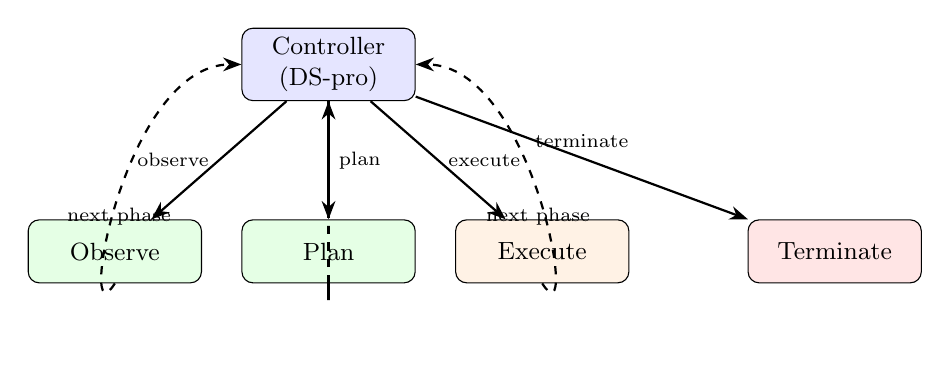
\begin{tikzpicture}[
    >=Stealth,
    box/.style={draw, rounded corners, minimum height=0.8cm,
                minimum width=2.2cm, align=center, font=\small},
    arrow/.style={->, thick},
  ]

  \node[box, fill=blue!10] (ctrl) {Controller\\(DS-pro)};
  \node[box, fill=green!10, below left=1.5cm and 0.5cm of ctrl]
    (obs) {Observe};
  \node[box, fill=green!10, below=1.5cm of ctrl]
    (plan) {Plan};
  \node[box, fill=orange!10, below right=1.5cm and 0.5cm of ctrl]
    (exec) {Execute};
  \node[box, fill=red!10, right=1.5cm of exec]
    (term) {Terminate};

  \draw[arrow] (ctrl) -- node[left, font=\scriptsize] {observe} (obs);
  \draw[arrow] (ctrl) -- node[right, font=\scriptsize] {plan} (plan);
  \draw[arrow] (ctrl) -- node[right, font=\scriptsize] {execute} (exec);
  \draw[arrow] (ctrl) -- node[above, font=\scriptsize] {terminate} (term);

  \draw[arrow, dashed] (obs.south) .. controls +(-0.5,-0.8) and
    +(-1.5,0) .. node[below, font=\scriptsize] {next phase} (ctrl.west);
  \draw[arrow, dashed] (plan.south) .. controls +(0,-0.8) and
    +(0,-1.5) .. node[below, font=\scriptsize] {} (ctrl.south);
  \draw[arrow, dashed] (exec.south) .. controls +(0.5,-0.8) and
    +(1.5,0) .. node[below, font=\scriptsize] {next phase} (ctrl.east);

\end{tikzpicture}
\caption{Controller loop. Each phase feeds back to the controller
for the next intent decision. Terminate exits the loop and returns
the final response.}
\label{fig:controller}
\end{figure}

%----------------------------------------------------------------------
\section{Backend--Tool Compatibility Matrix}
\label{sec:matrix}
%----------------------------------------------------------------------

\begin{table}[h]
\centering
\small
\begin{tabular}{@{}lcccccc@{}}
\toprule
\textbf{Backend} & \textbf{Native} & \textbf{XML}
  & \textbf{MCP} & \textbf{mesh-tool} & \textbf{Mesh Tools}
  & \textbf{Harness} \\
\midrule
\code{openai}       & \checkmark &            &            &             & \checkmark & via harness \\
\code{anthropic}    & \checkmark &            &            &             & \checkmark & via harness \\
\code{claude-code}  &            &            & \dag       & \checkmark  & \checkmark & via harness \\
\code{zai}          &            &            & \dag       & \checkmark  & \checkmark & via harness \\
\code{codex}        &            &            &            & \checkmark  & \checkmark & built-in \\
\code{mesh-harness} &            & \dag       &            & \checkmark  & \checkmark & \checkmark \\
\bottomrule
\end{tabular}
\caption{Backend--tool compatibility. ``Native'' = API-level function
calling. ``XML'' = \code{<mesh\_call>} in prompt. ``MCP'' = tools via
MCP sidecar. ``mesh-tool'' = tools via shell CLI. \dag~=~deprecated
path (still functional but being phased out). ``via harness'' =
available when the backend runs inside the harness layer.
\textbf{Key change}: codex now has mesh tool access via
\code{mesh-tool} CLI.}
\label{tab:matrix}
\end{table}

%----------------------------------------------------------------------
\section{Configuration Reference}
\label{sec:config}
%----------------------------------------------------------------------

\subsection{Backend Configuration (\code{mesh.yaml})}

Each backend is defined under \code{llm\_backends:} with at minimum:
\begin{lstlisting}
llm_backends:
  my-backend:
    backend_type: openai        # openai | anthropic | claude-code
                                # | zai | codex | mesh-harness
    api_key: ${ENV_VAR}
    base_url: https://...       # optional override
    default_model: gpt-5.1
    max_tokens: 16384
    temperature: 0.7
\end{lstlisting}

\subsection{Agent Node Configuration}

Each agent node under \code{nodes:} references a backend and specifies
tool access:
\begin{lstlisting}
nodes:
  agent:sysadmin:bob:
    nickname: bob
    llm_backend: claude-code-opus
    system_prompt_file: sysadmin.md
    tools: *common_tools           # YAML anchor
    memory_enabled: true
    memory_llm_backend: deepseek-direct
    memory_formation_v3_enabled: true
    memory_retrieval_redesign_enabled: true
\end{lstlisting}

\subsection{Harness Toolset Configuration}
\label{sec:harness-toolset}

The \code{mesh-harness} backend controls which tools the subprocess
receives via two config fields on \code{LLMConfig}:

\begin{itemize}[nosep]
  \item \code{harness\_toolset} (default: \code{"legacy"}) ---
        \code{"legacy"} exposes the full mesh tool set (email, calendar,
        notes, memory, browser, etc.\ via the parent agent's
        \code{ToolRegistry}); \code{"harness"} restricts to the 4-tool
        Codex-style surface (\code{file\_read}, \code{list\_dir},
        \code{grep}, \code{find\_files} plus \code{apply\_patch},
        \code{shell}).
  \item \code{harness\_tools} (default: \code{""}) --- comma-separated
        tool names. When non-empty, \emph{overrides}
        \code{harness\_toolset} entirely, giving fine-grained control.
\end{itemize}

\noindent
The toolset flag is passed to the subprocess via \code{-{}-toolset} or
\code{-{}-tools} CLI arguments (see \code{\_complete\_mesh\_harness()}
in \code{llm.py}).

\paragraph{Codex as direct backend vs.\ through harness.}
There is an important distinction between two ways an agent can use
Codex:
\begin{enumerate}[nosep]
  \item \textbf{Direct backend} (\code{backend\_type: codex}) ---
        \code{\_complete\_codex} launches the Codex CLI subprocess with
        its own built-in tools (\code{codex:shell}, \code{codex:patch},
        etc.).  Mesh tools are now available via \code{mesh-tool} CLI
        on \code{PATH} (repo root prepended to subprocess environment).
        The Codex agent calls \code{mesh-tool <name> -{}-args ...} from
        its shell tool.
  \item \textbf{Through harness} (\code{backend\_type: mesh-harness}
        with a codex sub-backend) --- the harness wraps the Codex model
        in its own TAOR loop and can expose mesh tools via
        \code{harness\_toolset: legacy}.  In this mode, mesh tools are
        available to the harness loop but the inner model does not see
        them directly.
\end{enumerate}

\subsection{Specialized LLM Clients}

Agents may use multiple LLM backends simultaneously:
\begin{itemize}[nosep]
  \item \textbf{Worker backend} (\code{llm\_backend}) ---
        primary LLM for conversation and tool use.
  \item \textbf{Router V2 backend} (\code{router\_v2\_llm\_backend}) ---
        separate LLM for the routing/classification layer.
  \item \textbf{Memory formation backend}
        (\code{memory\_llm\_backend}) --- dedicated LLM for the v3
        segmenter, decoupled from the worker backend (e.g.,
        \code{deepseek-direct} while the worker uses
        \code{claude-code-opus}).
  \item \textbf{Assessor backend} (in plan-and-execute) ---
        the controller/checkpoint LLM, configured per
        \code{mesh-harness} backend definition.
\end{itemize}

%----------------------------------------------------------------------
\section{Security Hardening}
\label{sec:security}
%----------------------------------------------------------------------

Several hardening measures protect subprocess spawning, credential
handling, and inter-process communication.

\subsection{Subprocess Environment Allowlist}

All LLM subprocess methods (\code{\_run\_cc\_subprocess},
\code{\_complete\_codex}, \code{\_complete\_mesh\_harness},
\code{cc\_session.py}, \code{router\_cc.py}, \code{eval/evaluator.py})
filter \code{os.environ} through \code{\_build\_subprocess\_env()}, a
module-level helper in \code{mesh/llm.py}. The allowlist is a
\code{frozenset} of~30 approved environment variables plus prefix
matching for \code{CLAUDE\_*} and \code{ANTHROPIC\_*}.

\begin{table}[h]
\centering
\small
\begin{tabular}{@{}lL{8cm}@{}}
\toprule
\textbf{Category} & \textbf{Allowed Variables} \\
\midrule
System     & \code{PATH}, \code{HOME}, \code{USER}, \code{SHELL},
             \code{LANG}, \code{LC\_*}, \code{TERM}, \code{TMPDIR},
             \code{XDG\_*}, \code{SSH\_AUTH\_SOCK} \\
API keys   & \code{OPENAI\_API\_KEY}, \code{ANTHROPIC\_API\_KEY},
             \code{DEEPSEEK\_API\_KEY}, \code{EXA\_API\_KEY},
             \code{ZAI\_API\_KEY}, \code{OPENROUTER\_API\_KEY},
             \code{SYNTHETIC\_API\_KEY}, \code{GOOGLE\_API\_KEY} \\
Mesh       & \code{MESH\_AUTH\_TOKEN}, \code{MESH\_NODE\_ID},
             \code{MESH\_ATTACHMENT\_SECRET} \\
Python     & \code{VIRTUAL\_ENV}, \code{PYTHONDONTWRITEBYTECODE},
             \code{PYTHONHASHSEED} \\
\bottomrule
\end{tabular}
\caption{Subprocess environment allowlist categories. Variables not in this
list (e.g., \code{LD\_PRELOAD}, \code{LD\_LIBRARY\_PATH},
\code{PYTHONPATH}) are blocked.}
\label{tab:env-allowlist}
\end{table}

\noindent
Operator-controlled overrides (\code{cc\_env}, \code{env\_override} in
\code{LLMConfig}) are applied \emph{after} filtering and may inject
arbitrary variables by design (e.g., account-specific \code{HOME},
custom API keys).

\subsection{API Key Masking in Logs}

The \code{\_mask\_cmd()} helper in \code{mesh/llm.py} masks sensitive
values in subprocess command logs. It handles both two-token
(\code{-{}-api-key VALUE}) and single-token (\code{-{}-api-key=VALUE})
forms, replacing values with \code{***} plus the last 4~characters.
Only log output is affected; the actual subprocess command is unchanged.

\subsection{Socket Path Hardening}

Agent tool sockets moved from the world-readable \code{/tmp/} directory
to \code{\textasciitilde/.mesh/sockets/} with directory mode~0700
(owner-only). Socket names are deterministic
(\code{\{sanitized\_node\_id\}.sock}) within the restricted directory---
no random suffix needed since only the owning user can list or connect.

\subsection{Node ID Propagation}

\code{MESH\_NODE\_ID} is set via two independent paths:
\begin{enumerate}[nosep]
  \item \textbf{Process-level}: \code{os.environ["MESH\_NODE\_ID"]}
        set in \code{AgentNode.\_\_init\_\_} for tool subprocess
        inheritance (\code{bash\_exec} uses \code{Popen} without
        explicit \code{env=}).
  \item \textbf{Per-LLMClient}: \code{LLMConfig.node\_id} injected
        explicitly into each LLM subprocess environment. Ensures
        correctness if multiple \code{LLMClient} instances exist in one
        process (main, memory, router backends).
\end{enumerate}

\subsection{Agent Node Refactoring}

The 842-line \code{\_process\_with\_llm} method was decomposed into a
280-line orchestrator plus six focused helpers:

\begin{itemize}[nosep]
  \item \code{\_setup\_controller\_for\_message} --- controller
        initialization and streaming observer.
  \item \code{\_build\_system\_prompt\_for\_llm} --- memory, preferences,
        personality, trace prompt assembly.
  \item \code{\_build\_worker\_instructions} --- worker instructions and
        briefing mode setup.
  \item \code{\_handle\_controller\_llm\_response} --- controller
        decision routing.
  \item \code{\_dispatch\_special\_tool\_calls} --- 10 special tool types
        (send\_message, schedule\_wake, etc.).
  \item \code{\_process\_tool\_calls\_in\_loop} --- full tool iteration
        processing with retry and error handling.
\end{itemize}

\subsection{IDLE$\to$BUSY Race Fix}

In \code{router\_v2.py}, the worker task is now created
\emph{before} \code{self.\_state} is set to \code{BUSY}. Since asyncio
is single-threaded, the task does not execute until the next yield, but
the invariant \code{\_state == BUSY $\implies$ \_worker\_task is not
None} now holds at every point.

%----------------------------------------------------------------------
\section{Memory System}
\label{sec:memory}
%----------------------------------------------------------------------

The memory system gives agents persistent, project-organized episodic
memory that survives across sessions. It operates at three layers:
conversation history (short-term), episodic memory pool (medium-term),
and project maps (structural).

\subsection{Architecture Overview}

\begin{figure}[h]
\centering
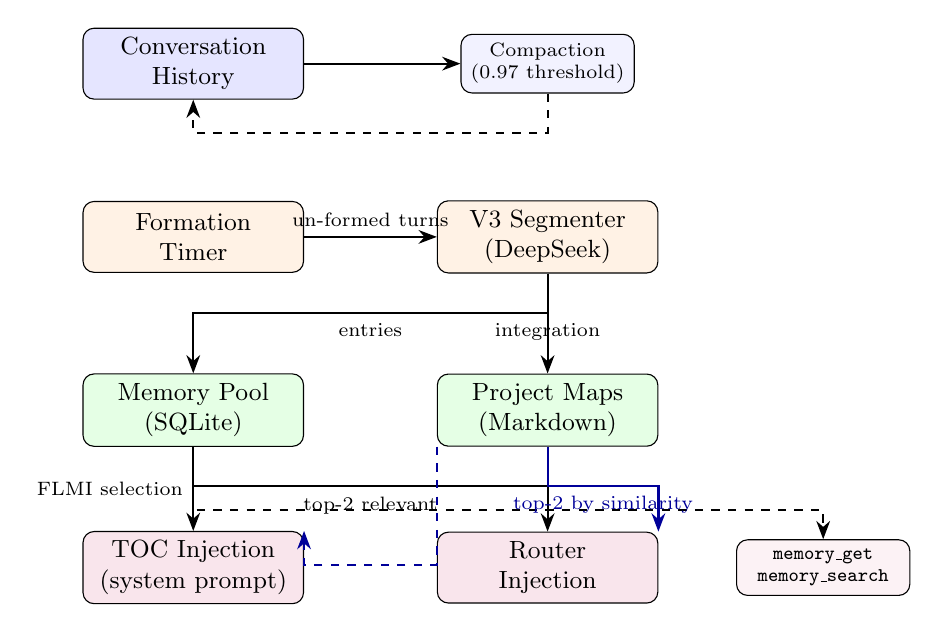
\begin{tikzpicture}[
    >=Stealth,
    box/.style={draw, rounded corners, minimum height=0.9cm,
                minimum width=2.8cm, align=center, font=\small},
    smallbox/.style={draw, rounded corners, minimum height=0.7cm,
                     minimum width=2.2cm, align=center,
                     font=\scriptsize},
    arrow/.style={->, thick},
    dasharrow/.style={->, thick, dashed},
    every node/.style={font=\small},
  ]

  % ── Row 0: Conversation ──
  \node[box, fill=blue!10] at (0, 0) (conv)
    {Conversation\\History};
  \node[smallbox, fill=blue!5] at (4.5, 0) (compact)
    {Compaction\\(0.97 threshold)};

  % ── Row 1: Formation pipeline ──
  \node[box, fill=orange!10] at (0, -2.2) (timer)
    {Formation\\Timer};
  \node[box, fill=orange!10] at (4.5, -2.2) (segmenter)
    {V3 Segmenter\\(DeepSeek)};

  % ── Row 2: Storage ──
  \node[box, fill=green!10] at (0, -4.4) (pool)
    {Memory Pool\\(SQLite)};
  \node[box, fill=green!10] at (4.5, -4.4) (maps)
    {Project Maps\\(Markdown)};

  % ── Row 3: Retrieval ──
  \node[box, fill=purple!10] at (0, -6.4) (toc)
    {TOC Injection\\(system prompt)};
  \node[box, fill=purple!10] at (4.5, -6.4) (router)
    {Router\\Injection};
  \node[smallbox, fill=purple!5] at (8, -6.4) (tools)
    {\code{memory\_get}\\
     \code{memory\_search}};

  % ── Arrows ──
  % Conversation → Compaction
  \draw[arrow] (conv) -- (compact);
  % Compaction feeds back
  \draw[arrow, dashed] (compact.south) -- ++(0,-0.5) -| (conv.south);

  % Timer → Segmenter
  \draw[arrow] (timer) -- node[above, font=\scriptsize]
    {un-formed turns} (segmenter);

  % Segmenter → Pool (entries)
  \draw[arrow] (segmenter.south) -- ++(0,-0.5) -|
    node[pos=0.25, below, font=\scriptsize] {entries} (pool.north);

  % Segmenter → Maps (integration)
  \draw[arrow] (segmenter.south) -- ++(0,-0.5) -|
    node[pos=0.25, below, font=\scriptsize]
    {integration} (maps.north);

  % Pool → TOC
  \draw[arrow] (pool) -- node[left, font=\scriptsize]
    {FLMI selection} (toc);

  % Pool → Router injection
  \draw[arrow] (pool.south) -- ++(0,-0.5) -|
    node[pos=0.25, below, font=\scriptsize]
    {top-2 relevant} (router.north);

  % Pool → tools
  \draw[dasharrow] (pool.south) -- ++(0,-0.8) -| (tools.north);

  % Maps → Router injection (relevance-based)
  \draw[arrow, blue!60!black] (maps.south) -- ++(0,-0.5) -|
    node[pos=0.25, below, font=\scriptsize, text=blue!60!black]
    {top-2 by similarity} (router.north east);

  % Maps → TOC (summary embeddings)
  \draw[dasharrow, blue!60!black] (maps.south west) -- ++(0,-1.5) -|
    (toc.north east);

\end{tikzpicture}
\caption{Memory system data flow. The formation timer drives the V3
segmenter, which produces entries persisted to the memory pool and
integrated into project maps. Retrieval surfaces memories via TOC
injection (always-on), router injection (per-dispatch), relevance-based
map injection (blue arrows, embedding similarity against recent turns),
and on-demand tools (\code{memory\_get}, \code{memory\_search}).}
\label{fig:memory}
\end{figure}

\paragraph{Three layers.}
\begin{description}[nosep, leftmargin=1.5em]
  \item[Conversation history] The raw message thread between user and
    agent. The router compacts it as context grows, using a forced
    synthesis threshold of 0.97 of the soft context limit. Recent
    messages stay intact; older turns are summarized. This provides
    short-term recall within a session.
  \item[Memory pool] Episodic memories stored in a SQLite database
    (\code{\textasciitilde/.mesh/memory/\{agent\}.db}). Each entry has
    three tiers of detail (Table~\ref{tab:memory-tiers}). The pool
    persists across sessions and grows over the agent's lifetime.
  \item[Project maps] Living Markdown summaries of each project's
    state---goals, architecture, key files, decisions, current status,
    and open issues. Stored centrally in
    \code{\textasciitilde/.mesh/memory/maps/\{project\_name\}.md}
    (constant \code{MAPS\_DIR} in \code{mesh/paths.py}) and indexed in
    the \code{project\_maps} SQLite table. A backward-compatibility
    migration copies legacy \code{PROJECT\_MAP.md} files to the central
    directory on first access.
\end{description}

\begin{table}[h]
\centering
\small
\begin{tabular}{@{}clL{7cm}@{}}
\toprule
\textbf{Tier} & \textbf{Name} & \textbf{Content} \\
\midrule
1 & Summary   & Short retrieval key (1--2 sentences). Always visible
                in the TOC. \\
2 & Reflection & Detailed analysis: what happened, why it matters,
                  lessons learned. Fetched via \code{memory\_get(id)}. \\
3 & Trace      & Full tool call trace from the original conversation.
                  Fetched via \code{memory\_get(id, full=true)}. \\
\bottomrule
\end{tabular}
\caption{Three-tier memory entry structure. Higher tiers are fetched on
demand to avoid context bloat.}
\label{tab:memory-tiers}
\end{table}

\subsection{Formation V3 Pipeline}

Memory formation converts un-formed conversation turns into structured
episodic entries. The V3 pipeline uses a dedicated LLM
(\code{memory\_llm\_backend}, typically \code{deepseek-direct}) that is
decoupled from the agent's primary worker backend.

\paragraph{Trigger and timing.}
Formation fires on two triggers:
\begin{enumerate}[nosep]
  \item \textbf{Timer}: a periodic timer (configurable interval, typically
        10--15~minutes) calls \code{form\_un\_formed()}.
  \item \textbf{Conversation boundary}: when the context window drops
        old turns during compaction, the dropped turns are processed
        via \code{on\_window\_drop()}.
\end{enumerate}

\paragraph{Segmenter.}
The V3 segmenter (\code{mesh/memory/formation\_v3.py}) sends un-formed
turns to the DeepSeek LLM with a structured prompt. The LLM returns a
JSON array of segments, each containing:

\begin{itemize}[nosep]
  \item \code{topic\_label} --- concise label for the segment.
  \item \code{summary} --- 2--3 sentence retrieval key.
  \item \code{reflection} --- detailed analysis and lessons learned.
  \item \code{project} --- project assignment (from known projects, or
        a suggestion if the project is new).
  \item \code{tags} --- categorization tags.
  \item \code{outcome} --- success, partial, or failure.
  \item \code{score} --- worthiness score (1--10; entries below~4 are
        filtered as ``not worth remembering'').
\end{itemize}

\paragraph{Cursor mechanics.}
A cursor index tracks which conversation turns have been processed.
Entry persistence and cursor advancement are atomic---if persistence
fails, the cursor stays put and the window is retried on the next
trigger. A cursor clamp (commit \code{a6f597d9}) prevents the cursor
from advancing past the actual history length after restarts.

\paragraph{Failure tolerance.}
A 3-strike system tracks per-window failures. After 3~consecutive
failures on the same window (keyed by \code{(cursor\_idx, end\_idx)}),
the window is skipped and the cursor advances past it. This prevents
a permanently stuck pipeline from blocking all future formation.

\paragraph{Cold-start handling.}
When no project maps exist, the segmenter is prompted to \emph{suggest}
project labels rather than requiring exact matches. The first entry
for a new project triggers \code{\_create\_new\_project\_map()}, which
bootstraps a skeleton map via a separate LLM call.

\subsection{Entry-Driven Map Curation}
\label{sec:map-curation}

After the V3 segmenter persists entries, a fire-and-forget
\code{asyncio.create\_task} integrates the new entries into their
respective project maps. This replaced the earlier conversation-driven
curation that ran in parallel with formation via
\code{asyncio.gather()}.

\paragraph{Flow.}
\begin{enumerate}[nosep]
  \item \code{form\_un\_formed()} persists entries and advances cursor.
  \item New-project bootstrap creates skeleton maps for unknown projects.
  \item \code{\_integrate\_entries\_into\_maps(entries)} is spawned as a
        background task:
  \begin{enumerate}[nosep]
    \item Group entries by \code{entry.project}, filtering empty projects.
    \item Per project: load current map, format entries with date,
          topic, score, outcome, tags, and summary.
    \item Send to DeepSeek LLM (\code{max\_tokens=32768}, 120s timeout)
          with the integration prompt.
    \item LLM produces \code{<section>} (full section replacement) and
          \code{<append\_to>} (append to section end) edit operations.
    \item \code{\_apply\_section\_updates()} parses and applies edits.
          Missing sections are created automatically.
  \end{enumerate}
\end{enumerate}

\paragraph{Design properties.}
\begin{itemize}[nosep]
  \item \textbf{Non-blocking}: integration failures are logged but do
        not affect entry persistence, cursor advancement, or the
        formation return value.
  \item \textbf{Multi-project}: a single formation batch may span
        multiple projects; each gets an independent integration call.
  \item \textbf{Composable with bootstrap}: new-project skeleton maps
        are created before integration runs, so the integrator always
        has a map to patch.
\end{itemize}

\paragraph{Canonical section schema.}
All three map prompts (curation, bootstrap, integration) reference the
same canonical section list, ensuring structural consistency across
creation and update paths:
\begin{enumerate}[nosep]
  \item \textbf{Summary} --- 2--3 sentences: what the project is, current phase.
  \item \textbf{Goals} --- what we are trying to accomplish, success criteria,
        guiding constraints. \emph{This is the single most important section.}
        When an agent must make a judgment call on an underspecified task,
        Goals is the anchor that keeps decisions aligned with project intent.
  \item \textbf{Architecture} --- system structure, data flow, key abstractions.
  \item \textbf{Key Files} --- navigational map with file paths, grouped by
        subsystem, with relationships noted (not a flat list).
  \item \textbf{Key Decisions} --- decisions made, rationale, dates.
  \item \textbf{Current State} --- what is active, completed, blocked, next.
  \item \textbf{Open Issues} --- unresolved problems, open questions.
  \item \textbf{Glossary} --- abbreviations, project-specific vocabulary.
\end{enumerate}
The integrator creates missing sections organically when entries reference
them---no migration of existing maps is needed.

\paragraph{Summary maintenance.}
Each project map has a short summary (1--2 sentences) stored alongside
an embedding vector in the \code{project\_maps} table. The summary
serves as the embedding target for relevance-based map injection
(\S\ref{sec:map-injection}). Summaries are extracted deterministically
after every map content change---via integration, tool edits, or manual
curation---by parsing the canonical \code{\#\# Summary} section from the
map content (no LLM call needed). If no \code{\#\# Summary} section
exists, the first non-heading paragraph (up to 500~characters) is used as
a fallback. The embedding is recomputed from the updated summary and
cached in memory. The update runs as a fire-and-forget
\code{asyncio.create\_task}, so it never blocks the caller.

\subsection{Retrieval}

Four retrieval paths surface memories and project context to the agent
at different points in the processing pipeline.

\subsubsection{TOC Injection (Always-On)}

The top~30 memory entries, ranked by relevance to the current
conversation, are injected as a \code{<memory\_toc>} block in the
agent's system prompt. Each entry shows its retrieval key (summary) and
ID. Entries already fetched this session are marked
\code{[already in context]}; entries injected into the current worker
dispatch are marked \code{[injected into worker]}.

\subsubsection{On-Demand Tools}

\begin{itemize}[nosep]
  \item \code{memory\_get(id)} --- fetches the full reflection (Tier~2)
        of a specific entry. The result persists in conversation history
        for the rest of the session---no re-fetching needed.
  \item \code{memory\_search(query, project=...)} --- semantic search
        over the memory pool using embedding similarity. Returns top-$k$
        entries. Use when the TOC doesn't surface what's needed.
\end{itemize}

\subsubsection{Router-Level Injection}

Before dispatching work to a worker, the router runs
\code{\_select\_memory\_context()} to curate and inject relevant
memories into the worker's context. The top~2 entries with a relevance
score above~0.3 are formatted as \code{<router\_injected\_context>} XML
and prepended to the worker's prompt. This ensures workers have relevant
historical context without requiring the agent to manually fetch
memories before each dispatch.

\subsubsection{Relevance-Based Map Injection}
\label{sec:map-injection}

Project maps are injected into both the router and worker prompts based
on relevance to the current conversation, replacing the earlier approach
of injecting only the statically-tracked \code{\_active\_project} map.

\paragraph{Algorithm.}
\begin{enumerate}[nosep]
  \item Concatenate the text of the last $N$ conversation turns
        ($N{=}5$ by default, hardcoded in the router's
        \code{\_get\_last\_n\_turns\_text()} helper).
  \item Embed the concatenated text using the memory embedding client
        (\code{text-embedding-3-small}).
  \item Compute cosine similarity between the context embedding and each
        project map's summary embedding (stored in the
        \code{project\_maps} table).
  \item Return the top-$k$ maps ($k{=}2$) with similarity above a
        minimum threshold (0.2).
\end{enumerate}

\paragraph{Injection points.}
\begin{itemize}[nosep]
  \item \textbf{Router prompt}: \code{\_build\_system\_prompt()} and
        \code{\_build\_router\_prompt()} call
        \code{render\_relevant\_maps\_block()} (which wraps
        \code{select\_relevant\_maps()}), injecting up to~2 maps as
        \code{<project\_map project="..." relevance="...">} blocks.
  \item \textbf{Worker prompt}: \code{\_select\_memory\_context()}
        appends relevant maps to the
        \code{<router\_injected\_context>} block alongside memory
        entries. Workers previously received no project maps.
  \item \textbf{Fallback}: if no map embeddings are available (embedder
        down, or maps lack summaries), falls back to
        \code{render\_maps\_block()} (active project only).
\end{itemize}

\paragraph{Summary embeddings.}
Each project map maintains a 1--2 sentence summary in the
\code{project\_maps.summary} column, extracted deterministically from
the map's \code{\#\# Summary} section after every content change
(\S\ref{sec:map-curation}). The summary is embedded via
\code{text-embedding-3-small} and stored in the \code{embedding} BLOB
column.
Summaries are better embedding targets than full map content: they
capture the project's domain and focus in a dense, semantically rich
form, whereas full maps contain structural/list content that dilutes
embedding quality.

\paragraph{Design rationale.}
The static \code{\_active\_project} approach had two limitations:
(1)~only one map was ever injected, even when conversations spanned
multiple projects, and (2)~workers received no project context at all.
Relevance-based selection aligns map injection with the same principle
used for memory entry retrieval---context earns its place in the prompt
by relevance, not by static assignment. The \code{\_active\_project}
field is retained for non-injection uses (formation defaults, TOC
project filtering, legacy curation paths).

\subsection{Selection and Weighting (FLMI)}

The active set (top~50 entries shown in the prompt TOC) is selected from
the full pool using Facility Location Mutual Information (FLMI), which
optimizes for \emph{embedding diversity}---ensuring broad coverage of
the agent's topic history rather than recency or frequency.

\paragraph{Selection mechanics.}
Each entry has an embedding vector (computed by the
\code{memory\_embedding\_backend}, typically OpenAI). FLMI evaluates
candidate swaps (new entry in, existing entry out) based on the
marginal diversity gain. Entries that improve coverage of
underrepresented topics are preferred.

\paragraph{Known issue: weight starvation.}
On agents with large pools (alice: 192~entries, ada: 135), FLMI's
diversity optimization means new V3 entries may receive weight~0 and
never enter the active set. The existing 50~entries already cover the
topic space, so new entries (which often overlap with recent work) offer
no diversity gain. This effectively fossilizes the active set.

\paragraph{Planned mitigation.}
A TOC redesign is under consideration: form the TOC via relevance to
the last $N$ messages (recency-aware), then apply FLMI within the
relevant subset if it exceeds the display budget. This would ensure
recent work is always represented while FLMI still provides diversity
within the relevant window.

\subsection{Feature Flag Matrix}

Memory features are deployed incrementally per agent via configuration
flags in \code{mesh.yaml}:

\begin{table}[h]
\centering
\small
\begin{tabular}{@{}lcccc@{}}
\toprule
\textbf{Agent} & \textbf{Formation V3} & \textbf{Retrieval Redesign}
  & \textbf{Trace-as-History} & \textbf{Memory LLM} \\
\midrule
bob (sysadmin)       & \checkmark & \checkmark &            & deepseek-direct \\
alice (assistant)     & \checkmark & \checkmark & \checkmark & deepseek-direct \\
hypatia (researcher)  & \checkmark & \checkmark &            & deepseek-direct \\
ada (researcher)      & \checkmark &            &            & deepseek-direct \\
gauss (researcher)    & \checkmark &            &            & deepseek-direct \\
eve (researcher)      &            &            &            & --- \\
reme (researcher)     &            &            &            & --- \\
\bottomrule
\end{tabular}
\caption{Memory feature deployment status per agent. Formation V3 uses
a dedicated DeepSeek LLM backend decoupled from the agent's worker
backend. Trace-as-history is off for most agents per operator directive.
Eve and reme have not been migrated to V3 or the retrieval redesign.}
\label{tab:memory-flags}
\end{table}

\subsection{Key Files}

\begin{table}[h]
\centering
\small
\begin{tabular}{@{}lL{7cm}@{}}
\toprule
\textbf{File} & \textbf{Purpose} \\
\midrule
\code{mesh/memory/system\_v2.py}
  & Core memory system: formation, curation, retrieval, FLMI selection,
    map management, relevance-based injection (~4000 lines). \\
\code{mesh/memory/formation\_v3.py}
  & V3 segmenter: JSON-structured LLM segmentation with validation,
    clamping, and retry logic. \\
\code{mesh/memory/store.py}
  & SQLite persistence: \code{MemoryEntry} dataclass, CRUD operations,
    embedding storage, project map storage. \\
\code{mesh/memory/selection.py}
  & FLMI active set selection using embedding vectors. \\
\code{mesh/memory/embeddings.py}
  & Embedding client for memory entry vectorization. \\
\code{mesh/paths.py}
  & Central path resolution: \code{MAPS\_DIR}
    (\code{\textasciitilde/.mesh/memory/maps/}), \code{MEMORY\_DIR},
    real-home bypass for CC agents. \\
\code{mesh/prompts/memory.md}
  & Shared prompt instructions for memory tools and TOC usage.
    Auto-appended to all agent prompts via \code{load\_prompt\_file()}. \\
\bottomrule
\end{tabular}
\caption{Memory system source files.}
\label{tab:memory-files}
\end{table}

\end{document}
